\documentclass[answers,addpoints]{exam} %answers,addpoints]{exam}

\usepackage{style}

\title{
    \vspace{-1cm}
	\horrule{1pt}\\[.5em]
	\huge Final Exam
	\horrule{2pt}
	\vspace{-1cm}
}
\author{}
\date{}

\begin{document}

\maketitle
    
\begin{center}
    \fbox{\fbox{\parbox{4.5in}{\centering Answer the questions in the spaces provided on the question sheets. If you run out of room for an answer, continue on the back of the page.}}}
\end{center}

\vspace{0.2in}
\makebox[\linewidth]{Name:\enspace\hrulefill } \\[2em]
\makebox[\linewidth]{Date:\enspace\hrulefill }

\vspace{1in}
\begin{center}
    \gradetable[h][pages]
\end{center}

\pagebreak

\begin{questions}

\section{Programming}

\question[5]

Humans have 10 fingers, so we decided to represent numbers in base 10. When we write down the number $312$, we are conveying the value 

$(\mathbf{3}\times 100) + (\mathbf{1} \times 10) + (\mathbf{2} \times 1)$

Computers don't have 10 fingers for counting. Instead, they essentially have 2 ``fingers", representing ``on" or ``off" voltage in their hardware. So instead of base 10 numbers, computers ``think" in base 2. When we write down the base 2 number $110_2$, we are conveying the value

$(\mathbf{1} \times 4) +( \mathbf{1} \times 2) + (\mathbf{0} \times 1)$

which is $6$ in base 10.

More generally, we can convert to decimal a base 2 number with three digits - a \textbf{left}, \textbf{middle}, and \textbf{right} digit - using the formula

$(\mathbf{left} \times 4) + (\mathbf{middle} \times 2) + (\mathbf{right} \times 1)$

\subsection{Part 1}
Write a program called BinaryToDecimal that has a user input 3 numbers representing a binary number. Calculate and print the decimal version of the binary number. Specifically, when you run the code for binary number $110_2$ it should look as follows: 

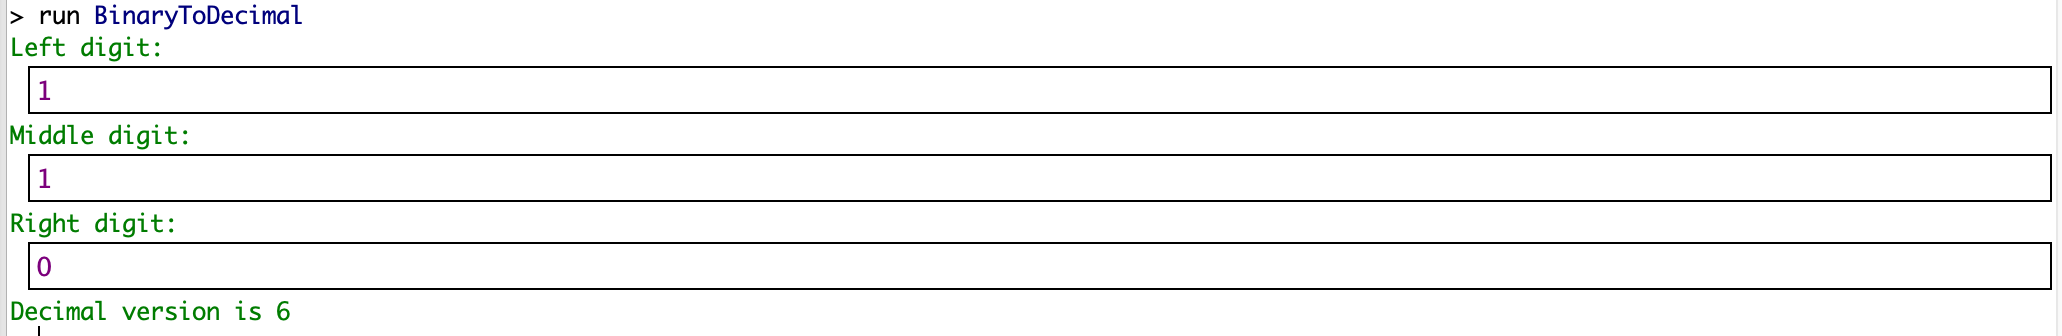
\includegraphics{binaryExample110}

For $010_2$, it should be 

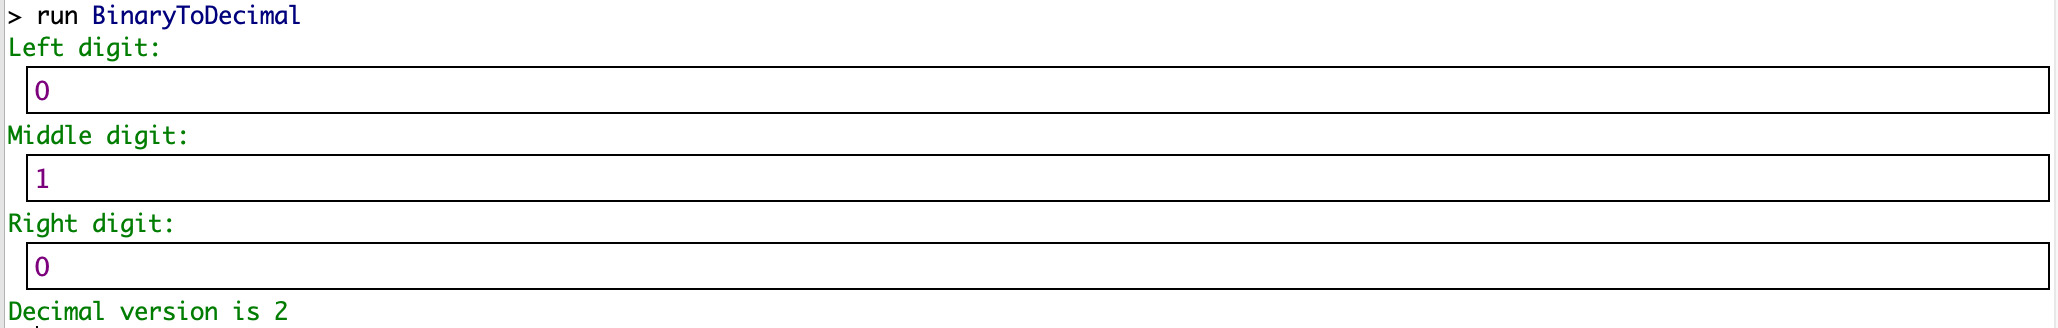
\includegraphics{binaryExample010}

\textbf{Suggested procedure}:

\begin{enumerate}

\item Start by copy/pasting old code - e.g. HelloPlanet.java, which already has a scanner set up - into a new Java file and just rename the class to $BinaryToDecimal$ and the file to $BinaryToDecimal.java$. Make sure the code runs before doing anything else. 

\item Modify the code to properly ask the user for the left, middle, and right digit (which are int types, not Strings), and put the user responses into appropriately named int variables. For now, just comment out the print statement. Run the code and make sure it matches the example output (other than giving the final answer). 

\item Now make a new variable for the final answer, and set its value using the formula in the intro for converting binary to decimal. Uncomment the print statement and modify it to print out the final answer with appropriate formatting. Test this code on both of the examples ($110_2$ and $010_2$) and make sure your code output looks exactly the same.

\end{enumerate}

\subsection{Part 2}

If you own or work at a software development company, writing the code is only the first step. Often you'll ``launch" your code (i.e. start selling it) only to have your ``users" (customers) start complaining about problems with the code. Software developers then need to code up a second version and relaunch, often calling it $V2$ for ``Version 2". 

In our case, we're writing a program to convert binary to decimal numbers but haven't checked that the user has input a proper binary number (which can only be made up of 0s and 1s). If the user inputs $150_2$, for example, the code will happily return 

$(\mathbf{1} \times 4) + (\mathbf{5} \times 2) + (\mathbf{0} \times 1)$

which is 9, despite that $150_2$ isn't a legal binary number so that this makes no sense. At least a few of our dumbest customers (and customers are always far dumber than software developers can imagine) will try getting the decimal version of non-binary numbers and will get mad at you when they're confused with a non-sense answer! But they're paying you, so let's give them a second version of the code that will write a message saying ``0s and 1s only!" if they attempt to type a number other than 0 or 1.

Write a program called BinaryToDecimalV2 that is an exact copy of BinaryToDecimal, but that now uses control structures to check each number as the user inputs them. Right after typing a bad number, print an error message. For example, if a user tries to type $150_2$, the output of the V2 code should be

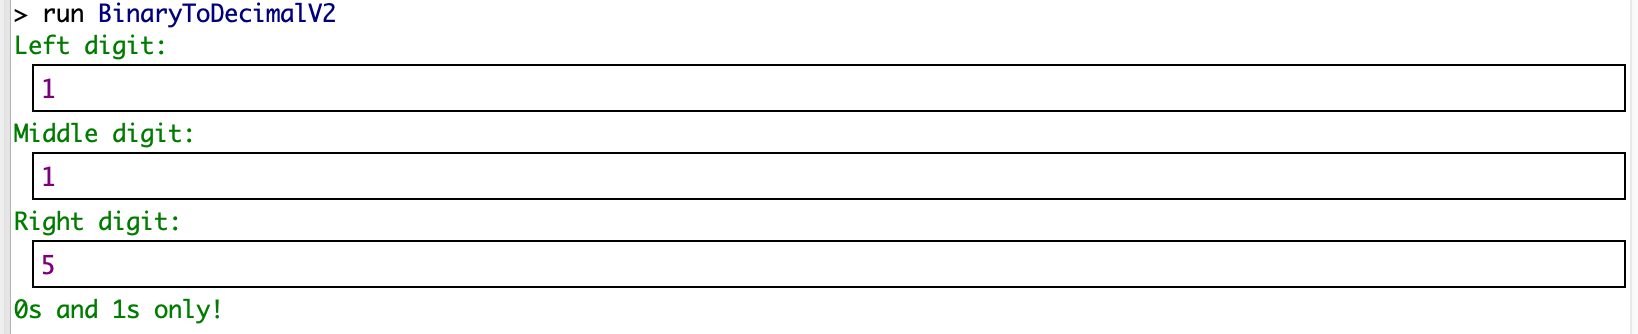
\includegraphics{binaryExampleError}

\textbf{Suggested procedure} 

\begin{enumerate}
\item As is good software development practice, before you start to code you should draw out your control structure flowchart, and explicitly write out the condition in code for each step. There are a couple different ways you can do this!

\item When you're ready with your hand-drawn flowchart, create a new file called BinaryToDecimalV2.java. Copy-paste in the code from BinaryToDecimal.java and rename the class from BinaryToDecimal to BinaryToDecimalV2. Make sure this compiles and runs before moving on. 

\item Now implement the first part of your control structure: check whether the first input number is 0 or 1, and print the error message if not. Run the regular code otherwise. Make sure this part works before moving on: test on at least one illegal case (e.g. $411_2$) and one legal case (e.g. $110_2$) before moving on. 

\item Now implement the rest of the control structure and test on a variety of legal and illegal cases, making sure it works as expected. 

\end{enumerate}

\begin{solution}

\begin{code}
import java.util.Scanner;

public class BinaryToDecimal {
  public static void main(String[] args) {  
    Scanner input = new Scanner(System.in);
    System.out.println("Left digit:");
    int leftDigit = input.nextInt();
    System.out.println("Middle digit:");
    int middleDigit = input.nextInt();
    System.out.println("Right digit:");
    int rightDigit = input.nextInt();
    input.close();
      
    int answer = leftDigit*4 + middleDigit*2 + rightDigit*1;
    System.out.printf("Decimal version is %d\n",answer);
  }
}
\end{code}

One possibility for V2: check each number one by one and throw an error at the moment the user types a bad one
\begin{code}
import java.util.Scanner;
class BinaryToDecimalV2 {
  public static void main ( String [] args ) {
    Scanner input = new Scanner(System.in);
    System.out.println("Left digit:");
    int leftDigit = input.nextInt() ; // get next user inputas a String
    if ((leftDigit==0) || (leftDigit==1)) {
      System.out.println("Middle digit:");
      int middleDigit = input.nextInt() ; // get next user inputas a String
      if ((middleDigit==0) || (middleDigit==1)) {
        System.out.println("Right digit:");
        int rightDigit = input.nextInt() ; // get next user inputas a String
        if ((rightDigit==0) || (rightDigit==1)) {
          int output = leftDigit*4+middleDigit*2+rightDigit;
          System.out.printf("Decimal version is %d\n", output ) ;
        }
        else {
          System.out.println("0s and 1s only!");
        }
      }
      else {
        System.out.println("0s and 1s only!");
      }
    }
    else {
      System.out.println("0s and 1s only!");
    }
    input.close() ; // close the Scanner
  }
}
\end{code}

Another possibility for V2: read all numbers in before checking any
\begin{code}
import java.util.Scanner;
class BinaryToDecimalV2 {
  public static void main ( String [] args ) {
    Scanner input = new Scanner(System.in);
    System.out.println("Left digit:");
    int leftDigit = input.nextInt() ; // get next user inputas a String
    System.out.println("Middle digit:");
    int middleDigit = input.nextInt() ; // get next user inputas a String
    System.out.println("Right digit:");
    int rightDigit = input.nextInt() ; // get next user inputas a String
    if ( ( (leftDigit==0) || (leftDigit==1) ) && 
        ( (middleDigit==0) || (middleDigit==1) ) &&
        ( (rightDigit==0) || (rightDigit==1) ) ) {
      int output = leftDigit*4+middleDigit*2+rightDigit;
      System.out.printf ("Decimal version is %d\n", output);
    }
    else {
      System.out.println("0s and 1s only!");
    }
    input.close() ; // close the Scanner
  }
}
\end{code}

\end{solution}

\pagebreak 

\question[15] 

If you have money in the bank, you can invest it to make more without doing any work! This is cynically part of why the rich get richer, but also an important finance tip. 

For example, if you have \$1,000 today and you use that \$1,000 to buy bonds that give you 10\% of the amount you have for every year you keep investing, that \$1,000 will grow larger. After the first year, you'll make $\$1,000 \times 10\%=\$1,000 \times 0.1=\$100$, giving you a total of \$1,100. So for the second year, you'll make $\$1,100 \times 10\% = \$1,100 \times 0.1 = \$110$, bringing your total amount of money up to \$1,210. In the third year, you'll make $\$1,210 \times 10\% = \$1,210 \times 0.1 = \$121$, bringing your total amount of money up to \$1331. Every year you make more money, and as time goes on the amount of money you make per year goes up since the interest ``compounds"! Mathematically speaking, the amount of money you have goes from \textbf{amount} to \textbf{amount + 0.1 * amount} every time a year passes. 

\subsection{Part 1}
Write a program called ``Interest" for a user to input the amount of money they have, and the number of years for which they'll invest it. Have the computer print how much money they'll have at the end of each year along the way, assuming a 10\%/year compounding interest rate. 

For the example we did above (invest \$1,000 for 3 years), the code should look exactly as follows when run: 

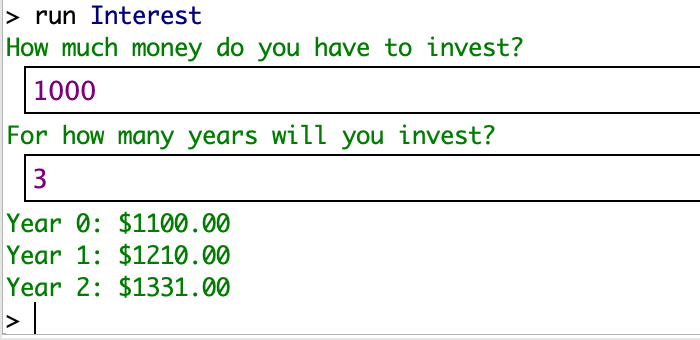
\includegraphics{interestExample}

\textbf{Suggested procedure}:

\begin{enumerate}

\item Start by copy/pasting old code - e.g. HelloPlanet.java, which already has a scanner set up - into a new Java file and just rename the class to $Interest$ and the file to $Interest.java$. Make sure the code runs before doing anything else. 

\item Modify the code to properly ask the user for the amount of money and the number of years (which are double and int types respectively, not Strings), and put the user responses into appropriately named variables. For now, just comment out the print statement. Run the code and make sure it matches the example output (other than giving the final answer). 

\item Now implement the formula, which will require you to use a for loop: for every year from 0 to the number of years for which the user is investing, update the amount of money the user has to be \textbf{amount + 0.1 * amount} then print the new amount with the proper formatting. Make sure you format the dollar outputs so there are exactly two decimal points!
\end{enumerate}

\subsection{Part 2}

We wrote a program to take in a number of years for which we'll invest, but we're not double checking that the user doesn't put in a negative number of years. As it stands, if a user types in a negative number to our program, the code will run and just print nothing without telling the user that they are only allowed to use a positive number of years.

Write a program called InterestV2 that is an exact copy of Interest, but that now uses a control structure to check whether the number of years is negative. If negative, print ``Error: can't enter negative number of years". Otherwise, run the code as before. Here is exactly what the output should look like if the user enters $-1$ number of years:

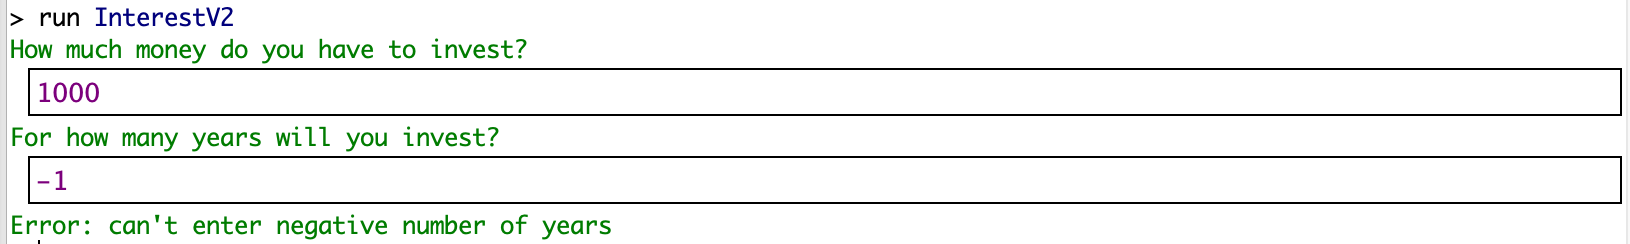
\includegraphics{interestExampleError}

\begin{solution}
\begin{code}
import java.util.Scanner; 

public class Interest {
  public static void main(String[] args) {
    // read in user values
    Scanner input = new Scanner(System.in);
    System.out.println("How much money do you have to invest?");
    double amount = input.nextDouble();
    System.out.println("For how many years will you invest?");
    int numYears = input.nextInt();
    input.close();
    
    if (numYears < 0) {
      System.out.println("Error: can't enter negative number of years");
    }
    else {
      for (int i=0; i<numYears; i++) {
        amount = amount + 0.1*amount; 
        System.out.printf("Year %d: $%.2f\n", i, amount);
      }
    }
  }
}
\end{code}

\begin{code}
import java.util.Scanner; 

public class Interest {
  public static void main(String[] args) {
    // read in user values
    Scanner input = new Scanner(System.in);
    System.out.println("How much money do you have to invest?");
    double amount = input.nextDouble();
    System.out.println("For how many years will you invest?");
    int numYears = input.nextInt();
    input.close();
    
    for (int i=0; i<numYears; i++) {
      amount = amount + 0.1*amount; 
      System.out.printf("Year %d: $%.2f\n", i, amount);
    }
  }
}
\end{code}

\end{solution}

\end{questions}

\end{document}
